\subsection{Citus: PostgreSQL Terdistribusi}

Citus merupakan mesin basis data terdistribusi untuk PostgreSQL yang menangani kebutuhan skalabilitas pada ekosistem PostgreSQL \parencite{citus}. Sebagai sebuah ekstensi, Citus menjaga kompatibilitas dengan PostgreSQL, sehingga dapat digunakan dengan PostgreSQL versi terbaru.

Sebuah kluster memiliki banyak \textit{node} yang terspesialisasi menjadi koordinator dan node pekerja. Aplikasi mengirimkan kueri kepada koordinator, lalu diteruskan kepada node pekerja terkait. Pendekatan ini memungkinkan setiap \textit{node} mampu memproses permintaan tulis sehingga pemrosesan bisa dilakukan secara parallel.

Selain itu, Citus memiliki skema \textit{sharding} berdasarkan skema dan baris. Hal ini diilustrasikan pada gambar \ref{fig:row-vs-schema-sharding}.

\begin{figure}[htbp]
    \centering
    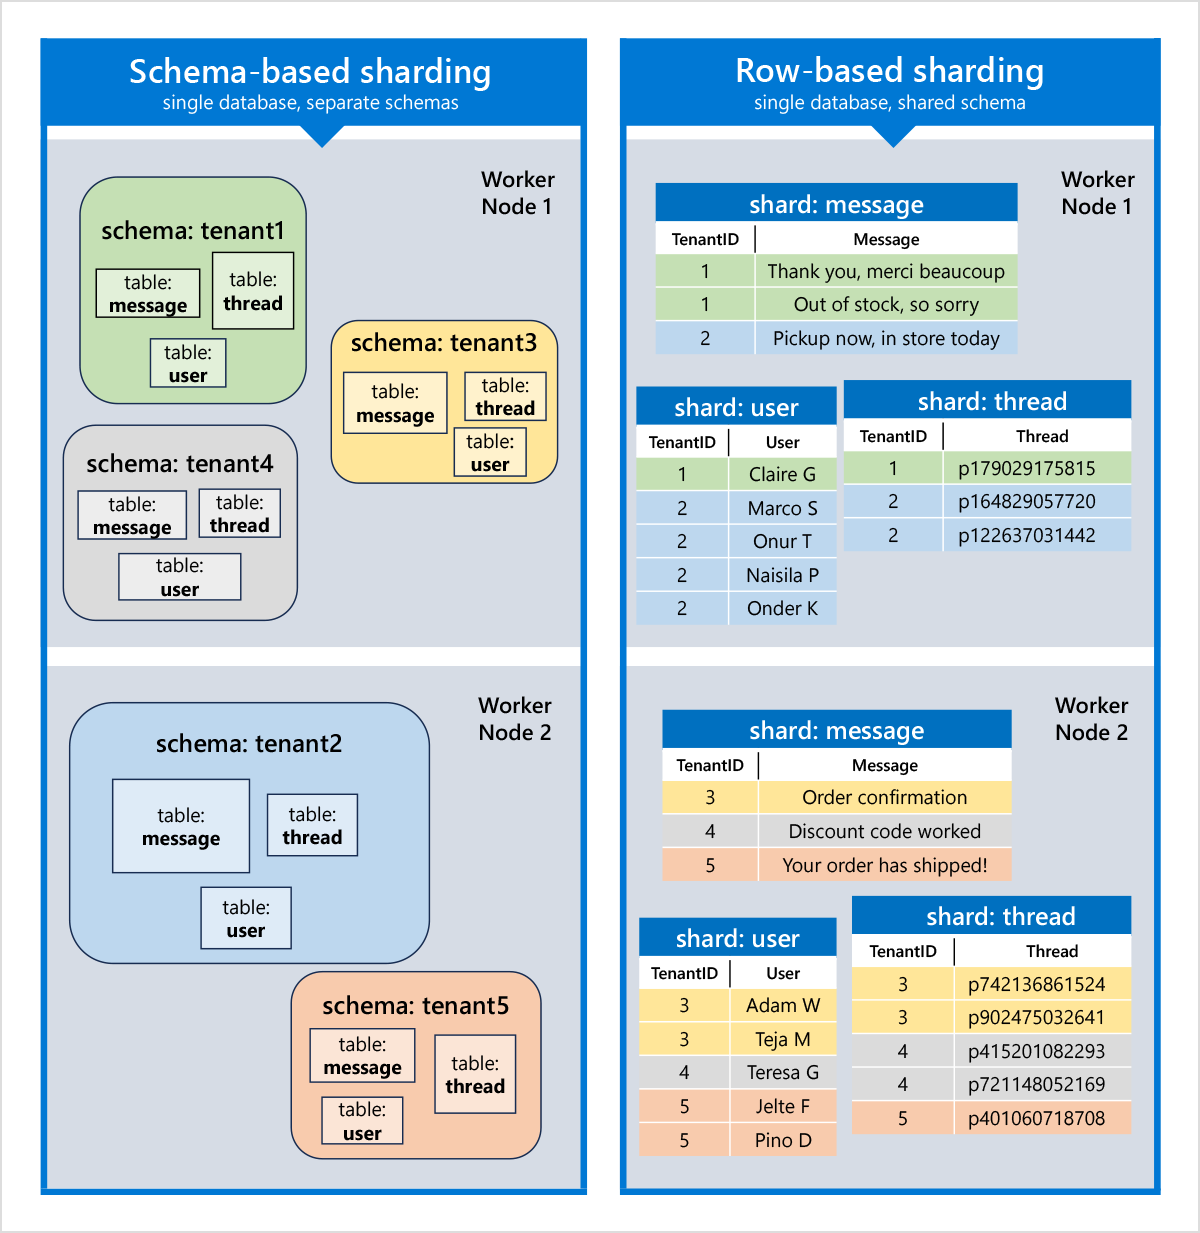
\includegraphics[width=0.6\textwidth]{resources/chapter-2/row-vs-schema-sharding.png}
    \caption{Perbandingan Pemartisian Data \parencite{schemaBasedSharding}}
    \label{fig:row-vs-schema-sharding}
\end{figure}

Selain itu, berikut adalah fitur lain ekstensi Citus:

\begin{enumerate}
    \item Tabel dibagi ke seluruh kluster node untuk menggabungkan sumber daya mesin (\textit{distributed tables}).
    \item Tabel referensi direplikasi ke seluruh node untuk kebutuhan penggabungan (\textit{join}) dan \textit{foreign key}, sehingga kinerja pembacaan data semakin baik (\textit{references tables}).
    \item Mesin kueri terdistribusi mengarahkan dan memparalelkan operasi pada tabel terdistribusi ke seluruh kluster.
    \item Model permartisian data berdasarkan baris dan berdasarkan skema.
\end{enumerate}
